% Instructions to change to html version:
% Comment out:
%  minipage, multicols,columnbreak, mathbf, hrule
% Replace all: \begin{minipage}% %%\end{minipage} %%%\begin{mulicols}  %%%\end{mulicols}  %%\columnbreak % %%\begin{framed} %%%\end{framed} %%%\hrule
% Search for \mathbf
% Replace \\] with \[ and \) with \(
% Enclose graphics in figure environments and add captions
% Re-tag \df environments as sections, subsections, etc.
% Command Line Code to Create html version:
%First: pdflatex -shell-escape filename.tex                                   
%Second, for each figure: inkscape "filename-figure1.pdf" -o "filename-figure1.png"
% Third: htlatex filename.tex "ht5mjlatex.cfg, charset=utf-8" " -cunihtf -utf8"


\documentclass[10pt]{article}

%\usepackage{tikz, pgf,pgfplots,wasysym,array}
%\usepackage{wasysym,array}

\usepackage{amsmath,amssymb}

\ifdefined\HCode
  \def\pgfsysdriver{pgfsys-tex4ht-updated.def}
\fi 
%\ifdefined\HCode
%  \def\pgfsysdriver{pgfsys-dvisvgm4ht.def}
%\fi 
\usepackage{tikz}
\usetikzlibrary{calc,decorations.markings,arrows}
\usepackage{pgfplots}

\pgfplotsset{compat=1.12}
\usepackage{myexternalize}
\usetikzlibrary{calc,decorations.markings,arrows}
\usepackage{framed}
\usepackage[none]{hyphenat}

\input{../../../common/1336_header_test.tex}

\begin{document}

\everymath{\displaystyle}



\newcommand{\ihat}{\boldsymbol{\hat{\textbf{\i}}}}
\newcommand{\jhat}{\boldsymbol{\hat{\textbf{\j}}}}
\newcommand{\khat}{\boldsymbol{\hat{\textbf{k}}}}

\let\oldvec\vec
%\renewcommand{\vec}[1]{\oldvec{\mathbf{#1}}}

\renewcommand{\u}{\vec{u}}
\renewcommand{\v}{\vec{v}}
\newcommand{\w}{\vec{w}}
\renewcommand{\r}{\vec{r}}
\renewcommand{\a}{\vec{a}}
\renewcommand{\b}{\vec{b}}

\newcommand{\grad}{\vec{\nabla}}
\newcommand{\<}{\left\langle}
\renewcommand{\>}{\right\rangle}

\renewcommand{\myTitle}{MATH 2330: Multivariable Calculus}

\renewcommand{\mySubTitle}{Chapter 6 - Part 3}
%~\hfill Name: \underline{~~~~~~~~~~~~~~~~~~~~~~~~~~~~~~~~~~~~~~~~~~~~~~~}

\lectTitle{\vspace*{-.5in}\myTitle}{\vspace*{.1in}\mySubTitle \vspace*{-.25in}}



\section*{6.3 - The Fundamental Theorem of Calculus for Line Integrals (FTCFLI), Part 2:}


\hspace*{-.8in}%\begin{minipage}{1.25\textwidth}
%\begin{framed}



\subsection*{FTCFLI:}
If \(f\) is differentiable and \(\grad f\) is continuous on a curve \(C\) parametrized as \(\vec{r}(t)\) for \(a\leq t \leq b\), then

\[
\int_C \grad f \cdot d\vec{r} = f(\vec{r}(b)) - f(\vec{r}(a)).
\]

This means that if \(\vec{F}=\grad f\) for some potential function \(f\) then the line integral \(\int_C \vec{F}\cdot d\vec{r}\) is path independent.

\vspace*{.1in}%\hrule \vspace*{.2in}

\subsection*{Properties of Conservative Vector Fields:}


\(\vec{F} = \<P(x,y), Q(x,y)\>\) is conservative on a region \(R\) in the plane (with no holes) if:
\begin{enumerate}[A:]

\item \(\oint_C \vec{F}\cdot d\vec{r} = 0\) for any closed path \(C\)
\item \(\int_C \vec{F}\cdot d\vec{r}\) depends only on the endpoints, not on the path itself
\item \(\vec{F} = \grad f\) for some potential function \(f\)
\item The components satisfy the \textbf{component test}:
\(
\frac{\partial P}{\partial y} = \frac{\partial Q}{\partial x}
\)

\end{enumerate}

%\end{framed}

%\end{minipage}

\section*{Problems for Group Work:}


\begin{enumerate}[{Problem} 1: ]
%\addtocounter{enumi}{1}
\item The following vector fields are conservative. For each one, find the potential function, \(f\) such that \(\vec{F} = \grad f\):
\begin{enumerate}[a)]
\item \(\vec{F} = \<3xy^2, 3x^2y\>\)
\item \(\vec{F} = y\sin(xy)\ \ihat +x\sin(xy)\ \jhat\)
\item \(\vec{F} = (2x+y)\ \ihat +(x+3y^2)\ \jhat\)
\item \(\vec{F} = \<yze^{xyz},xze^{xyz},xye^{xyz}\>\)

\end{enumerate}

\item Which, if any, of the following vector fields are conservative? \label{VFs}
\begin{enumerate}[a)]
\item \(\vec{F} = xy\ \ihat -2xy\ \jhat\)
\item \(\vec{F} = (2xy+\cos(2y))\ \ihat +(x^2-2x\sin(2y))\ \jhat\)
\item \(\vec{F} = (3x-5y)\ \ihat +(7y-5x)\ \jhat\)

\end{enumerate}

\item Evaluate \(\oint_C\vec{F}\cdot d\vec{r}\) for each of the vector fields from Problem \ref{VFs}, for the curve \(C\): \(x^2+y^2=1\), oriented counter-clockwise.

\end{enumerate}

\pagebreak

\section*{6.4 - Green's Theorem:}

\hspace*{-.8in}%\begin{minipage}{1.25\textwidth}
%\begin{framed}

\subsection*{Green's Theorem:}


%\begin{minipage}{.3\textwidth}


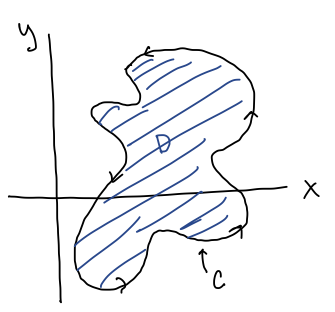
\includegraphics[width=\textwidth]{Ch13s4-GT.png}

%\end{minipage}
\hspace*{.4in}
%\begin{minipage}{.6\textwidth}

For any vector field \(\vec{F} = \<P,Q\>\) that has continuous first partials:

\[
\oint_C \vec{F}\cdot d\vec{r} = \oint_C P\ dx + Q\ dy = \iint_D \frac{\partial Q}{\partial x} - \frac{\partial P}{\partial y} \ dA,
\]

where \(C\) is a \textbf{simple closed curve} that is \textbf{piecewise smooth} and \textbf{positively oriented} that encloses the region \(D\).

\begin{itemize}
\item \textbf{simple closed curve:} only intersects itself at the start/end points
\item \textbf{piecewise smooth:} can be broken up into pieces without corners
\item \textbf{positively oriented:} draw the arrows on \(C\) sot that the enclosed region \(D\) is always on the left as you go around \(C\).

\end{itemize}

%\end{minipage}


\vspace*{.1in}%\hrule \vspace*{.2in}

\subsection*{Area Formulas:}

Green's Theorem can be used to calculate the area of the region \(D\) by choosing \(P\) and \(Q\) so that \(\frac{\partial Q}{\partial x} - \frac{\partial P}{\partial y}=1\).\\ The most popular options are shown below:
\[
\text{Area}(D) = \oint_C x\ dy = -\oint_C y\ dx = \frac{1}{2}\oint x\ dy - y\ dx.
\]
Use whichever formula makes the problem the easiest!

%\end{framed}

%\end{minipage}

\section*{Examples:}


\begin{enumerate}[{Example} 1: ]

\item \textbf{Making the tedious...less tedious!}\\
Evaluate \(\oint_C x^2y\ dx + (x^3+2xy^2)\ dy\), where \(C\) encloses the region between the unit circle and the circle with radius 2 in quadrants IV and I.
\vfill


\item \textbf{Making the Impossible Possible!}\\
Evaluate the line integral
\[
\oint_C \left(2y+\sqrt{1+x^5}\right)\ dx + \left(5x-e^{y^2}\right)\ dy,
\]
where \(C\) is the ``unit square'' connecting the points \((-\tfrac{1}{2},-\tfrac{1}{2})\), \((-\tfrac{1}{2},\tfrac{1}{2})\), \((\tfrac{1}{2},\tfrac{1}{2})\), and \((\tfrac{1}{2},-\tfrac{1}{2})\)


\vfill

\item \textbf{Area of the Astroid!}\\
Use Green's Theorem to find the area enclosed by the astroid: \(\vec{r}(t) = \< \cos^3 t, \sin^3 t\>\), \( 0\leq t\leq 2\pi\).

\vfill

\end{enumerate}

\end{document}